% Sección de aprendizaje automático de la memoria conjunta del TFM.
% Versión 7 (14/09/2026): la memoria de la v6 y un anexo breve con enlaces
% al repositorio. pdflatex seccion_ML_v7.tex (dos pasadas). Figuras en figs/.
\documentclass[10pt,a4paper]{article}

\usepackage[T1]{fontenc}
\usepackage[utf8]{inputenc}
\usepackage{lmodern}
\usepackage[margin=1.55cm]{geometry}
\usepackage{graphicx}
\usepackage{booktabs}
\usepackage{array}
\usepackage{caption}
\usepackage{microtype}
\usepackage{enumitem}
\usepackage[section]{placeins}
\usepackage{amsmath}
\usepackage{float}
\usepackage{tikz}
\usetikzlibrary{arrows.meta,positioning}
\usepackage[hidelinks]{hyperref}

\graphicspath{{figs/}}
\captionsetup{font=small,labelfont=bf,skip=4pt,width=.92\textwidth}
\captionsetup[table]{labelsep=period}
\setlist{nosep,leftmargin=*}
\setlength{\parskip}{0.2em}
\linespread{0.97}
\setlength{\emergencystretch}{2em}
\renewcommand{\figurename}{Figura}
\renewcommand{\tablename}{Tabla}
\renewcommand{\thesubsection}{\arabic{subsection}}

\begin{document}


\section*{Predicción diaria del riesgo de incendio: dónde y cuándo}
\label{sec:ml}

\subsection{Objetivo y resultado}

La España peninsular y Baleares se representan en 498,530 celdas de un
kilómetro de lado. El objetivo de este módulo es ordenar cada mañana esas
celdas de mayor a menor riesgo de incendio para el día en curso. Su calidad se mide con un solo criterio: si las celdas que ardieron
ese día ocupaban las primeras posiciones. Dentro del sistema conjunto, este
módulo cubre el 'antes' del incendio. La visión por computador cubre el
'durante' y el asistente sobre los partes del MITECO (Ministerio para la
Transición Ecológica y el Reto Demográfico), la consulta.

El trabajo se desarrolló en dos iteraciones. Un primer modelo alcanzó un AUC
(\emph{Area Under the ROC Curve}) de 0.89 en su conjunto de prueba. Puesto en
producción y evaluado contra la superficie quemada real, obtuvo entre 0.57 y
0.64. El problema no era el algoritmo ni el clima. El modelo respondía a una pregunta que no interesaba, dejando la verdadera cuestión sin resolver. Con el diseño corregido, el segundo modelo pasó de 0.74 a 0.81 en
la temporada de 2025 y de 0.66 a 0.76 en la de 2026, evaluado día a día sobre
las dos temporadas completas.

\subsection{Datos}

Se emplearon cuatro fuentes, descritas en el anexo~A:

\begin{itemize}
  \item IberFire, un cubo de datos abierto (Tekniker y UPV/EHU, Universidad
  del País Vasco / Euskal Herriko Unibertsitatea). Contiene 261 variables
  diarias por celda de 1~km entre 2008 y 2024: meteorología, vegetación,
  relieve, usos del suelo, población y carreteras. De él proceden casi todas
  las variables del modelo.
  \item EGIF (Estadística General de Incendios Forestales), el registro
  oficial de incendios del Ministerio. Tiene una fila por incendio, con su
  fecha y el punto de inicio. Es la etiqueta del primer modelo.
  \item EFFIS (\emph{European Forest Fire Information System}), los perímetros
  de superficie quemada que Copernicus cartografía por satélite. Es la
  etiqueta del segundo modelo y la verdad contra la que se evalúan los dos.
  \item ERA5-Land (\emph{ECMWF Reanalysis v5 Land}) e IFS (\emph{Integrated
  Forecasting System}), ambos del ECMWF (\emph{European Centre for
  Medium-Range Weather Forecasts}). El primero es el reanálisis meteorológico,
  que describe lo ocurrido; el segundo es la previsión. Se entrena con el
  reanálisis y se sirve con la previsión. El primer modelo se sirvió con la
  observación de 687 estaciones de AEMET (Agencia Estatal de Meteorología).
\end{itemize}

A partir de estas fuentes se construyen 46 variables por celda y día, en
cuatro familias. La meteorología: temperatura, humedad, viento, precipitación
del día y de los últimos 7, 15 y 30 días, y el índice de peligro FWI
(\emph{Fire Weather Index}). Las características de la celda: bosque,
matorral, pendiente, altitud, carreteras y población. El historial de fuego
del entorno: incendios a 1 y 10~km en meses y años anteriores, y focos
térmicos de satélite en la última semana. Y el calendario.

El análisis exploratorio aportó tres resultados principales. El primero es la escasez del fenómeno. En la mayoría de los veranos de 2015 a
2024 hubo entre 2 y 7 celdas ardiendo por cada 100,000 al día, según los
perímetros de EFFIS. Además, solo el 3~\% de las celdas registró alguna ignición
entre 2015 y 2020, según la EGIF.

El segundo es la agrupación espacial. Las celdas quemadas son contiguas,
porque proceden de perímetros. Por eso una partición aleatoria entre
entrenamiento y prueba aumenta el AUC, por esto se hicieron las particiones del trabajo por bloques de 100~km o por años.

El tercero afecta al FWI. Su valor absoluto toma valores de significado distinto según el
lugar: un FWI de 40 es habitual en Almería y excepcional en Asturias. Lo que
separa los días con fuego es lo inusual que resulta ese valor en cada celda.
Por ello el FWI se expresa como percentil respecto a la historia de la propia
celda. En el conjunto de entrenamiento, la mediana de ese percentil es 84 en
los días con fuego y 47 en los días sin fuego.

\subsection{Primer modelo: entrenamiento y evaluación en operación}

El primer modelo se construyó con el diseño habitual en la literatura. Los
positivos fueron los 19,561 incendios del registro EGIF entre 2015 y 2020,
cada uno en su celda y su fecha. Los negativos se tomaron de la misma celda en
otros días sin incendio, tres por cada positivo. Se entrenó un modelo XGBoost
(\emph{eXtreme Gradient Boosting}) y se ajustó con los datos de 2021. Se probó
con los de 2022, el peor año de la década, que incluye los incendios de
Losacio y la Sierra de la Culebra. El resultado fue un AUC de 0.89. No había
fugas de información (con las etiquetas barajadas el modelo cae al azar) ni
pérdida apreciable al validarlo por bloques espaciales de 100~km. El ajuste de
hiperparámetros añadió solo +0.007, por lo que el rendimiento procedía de las variables.

Con ese resultado, el modelo se puso en producción en julio de 2026. Cada
mañana descarga la observación de las 687 estaciones, calcula las 46 variables
y publica un ranking nacional y un mapa de riesgo para el día y el siguiente.
Desde entonces se ejecuta a diario.

La evaluación se hizo contra tres fuentes de datos independientes: los perímetros de
EFFIS, los partes diarios del MITECO y los focos térmicos de satélite. El
acierto diario del modelo en producción se situó entre 0.57 y 0.64. Un índice
sin modelo, el percentil local del FWI, alcanzó 0.70. Se consideraron tres
explicaciones, y las dos primeras se descartaron:

\begin{enumerate}
  \item La medida no era el problema. Las tres verdades, procedentes de
  satélite, de cartografía y de partes oficiales, coincidían.
  \item La meteorología tampoco. El modelo se entrenó con el reanálisis del
  cubo y se sirve con estaciones, y hay diferencias reales entre las dos
  fuentes: el reanálisis registra 8~mm más de lluvia al mes, lo que reduce el
  FWI en 10 puntos. Cuantificadas, esas diferencias no explican la caída.
  Tampoco la explica lo que cambia entre entrenamiento y servicio: sustituir
  las variables de satélite por su climatología cuesta 0.0045 de AUC.
  \item La causa estaba en la pregunta. Al tomar los negativos de la misma
  celda en otros días, el 98.8~\% de las celdas de la muestra tenía exactamente
  un 25~\% de días con fuego. Con la misma proporción en todas las celdas, el
  modelo no podía aprender qué celda es más peligrosa que otra; solo podía
  aprender qué día lo es. El modelo respondía a «¿es hoy un día peligroso en
  esta celda?». En operación se le preguntaba «¿cuál de las 498,530 celdas
  arde hoy?».
\end{enumerate}

\subsection{Segundo modelo: mismo algoritmo, distinta pregunta}

Se comienza analizando la figura~\ref{fig:disenios} que resume el problema y su solución. En el primer
diseño (a), cada celda quemada se compara consigo misma en otros días. En el
segundo (b), se compara con otras celdas del mismo día, que es lo que se pide
en operación (c). La prueba de que ese era el fallo es que la métrica de
laboratorio no lo detectaba. Dos conjuntos de entrenamiento, uno con cada
diseño, obtuvieron 0.92 medidos cada uno con su propio conjunto de prueba.
Medidos dentro de cada día, como se usan, obtuvieron 0.744 y 0.828.

\begin{figure}[htbp]
  \centering
  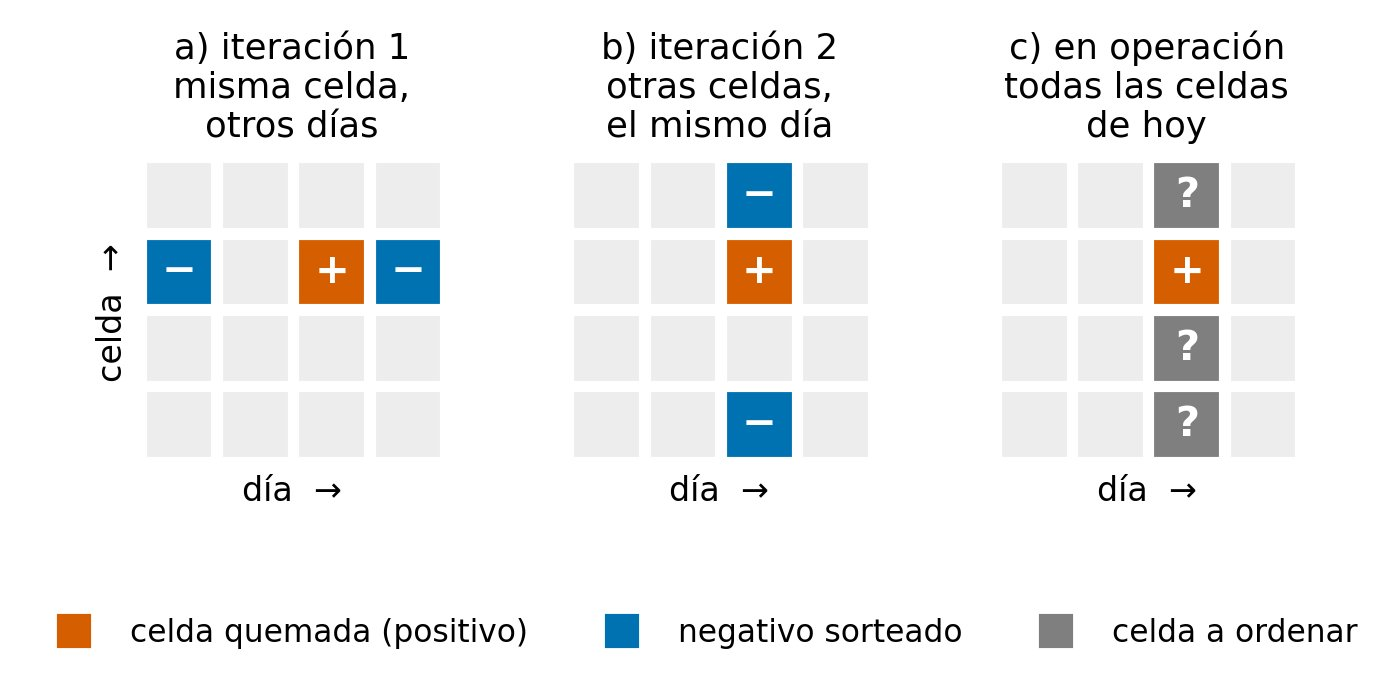
\includegraphics[width=.58\textwidth]{pagina_2_imagen_1_Im0.jpg}
  \caption{La misma rejilla celda~$\times$~día con los dos diseños de muestreo
  y la pregunta operativa. (a)~Primera iteración: para cada celda quemada, los
  negativos son la misma celda en otros días, y el modelo solo puede aprender
  qué día es peligroso. (b)~Segunda iteración: los negativos son otras celdas
  del mismo día, y el modelo aprende a comparar celdas. (c)~Lo que se pide
  cada mañana: ordenar todas las celdas del día. Solo (b) plantea la misma
  pregunta que (c).}
  \label{fig:disenios}
\end{figure}

La segunda versión cambió dos elementos y mantuvo el resto: las mismas 46
variables, el mismo algoritmo con los mismos hiperparámetros y la misma malla.
Los negativos pasaron a ser otras celdas del mismo día. La etiqueta pasó a ser
la superficie quemada de EFFIS, la misma con la que se evalúa. Este segundo
cambio responde a una comprobación previa: solo el 15~\% de las igniciones de
EGIF de entre 25 y 100 hectáreas coincidía, en la misma celda y fecha, con un
perímetro de EFFIS. Entrenar con puntos de ignición y evaluar con perímetros
equivalía a comparar dos magnitudes distintas.

Con el nuevo diseño se entrenó con los años 2015 a 2022, se ajustó con 2023 y
se probó con 2024, siempre evaluando dentro de cada día. Se compararon dos
alternativas: un modelo único, y la combinación de un modelo de «dónde»
(estático) con otro de «cuándo» (diario). También se probaron distintas
cantidades de negativos por positivo. Se eligió el modelo único con diez
negativos por positivo, denominado r10 en adelante.

La elección se apoyó en la temporada de 2026, externa al cubo y con 74 días con
fuego. Frente a la pareja, el modelo único ordenó mejor las celdas de cada día:
0.752 frente a 0.705 de AUC medio. En la prueba de 2024 la pareja había quedado
por delante (0.840 frente a 0.809), pero perdió esa ventaja en 2026. Frente a otras cantidades de negativos, el acierto medio apenas cambió,
entre 0.745 y 0.759, del orden del ruido del sorteo. Diez negativos por positivo
situaron mejor los incendios grandes: el percentil medio de las celdas quemadas,
ponderado por hectáreas, pasó de 79.5 con tres negativos a 81.9 con diez. La
reproducción posterior de las temporadas de 2025 y 2026 confirmó la elección. De
los seis modelos comparados, el r10 obtuvo el mayor AUC medio en las dos, con un
protocolo de evaluación fijado por escrito antes de ejecutarla.

Las pruebas con resultado negativo se recogen en el
anexo~B: entrenar solo con verano y añadir una capa de 'ya quemado' empeoran
el modelo.

Antes de dar por bueno el modelo se comprobó en qué variables se apoya y si
eso concuerda con lo que se sabe del fuego (figura~\ref{fig:shap}). La
variable de mayor peso es el historial: el número de incendios a 10~km en el
mismo mes de años anteriores. Le siguen el combustible (verdor acumulado en el
último mes, matorral y pendiente) y la meteorología.

Una humedad mínima baja y
un FWI anómalo para la celda elevan el riesgo; el suelo agrícola y la lluvia
reciente lo reducen. El verdor y la temperatura de superficie del propio día contienen ya
parte de la firma del incendio en el cubo, y suponen un 4~\% del peso del
modelo. En servicio se sustituyen por su climatología mensual, porque no fue
posible disponer de ellos en producción.

\begin{figure}[htbp]
  \centering
  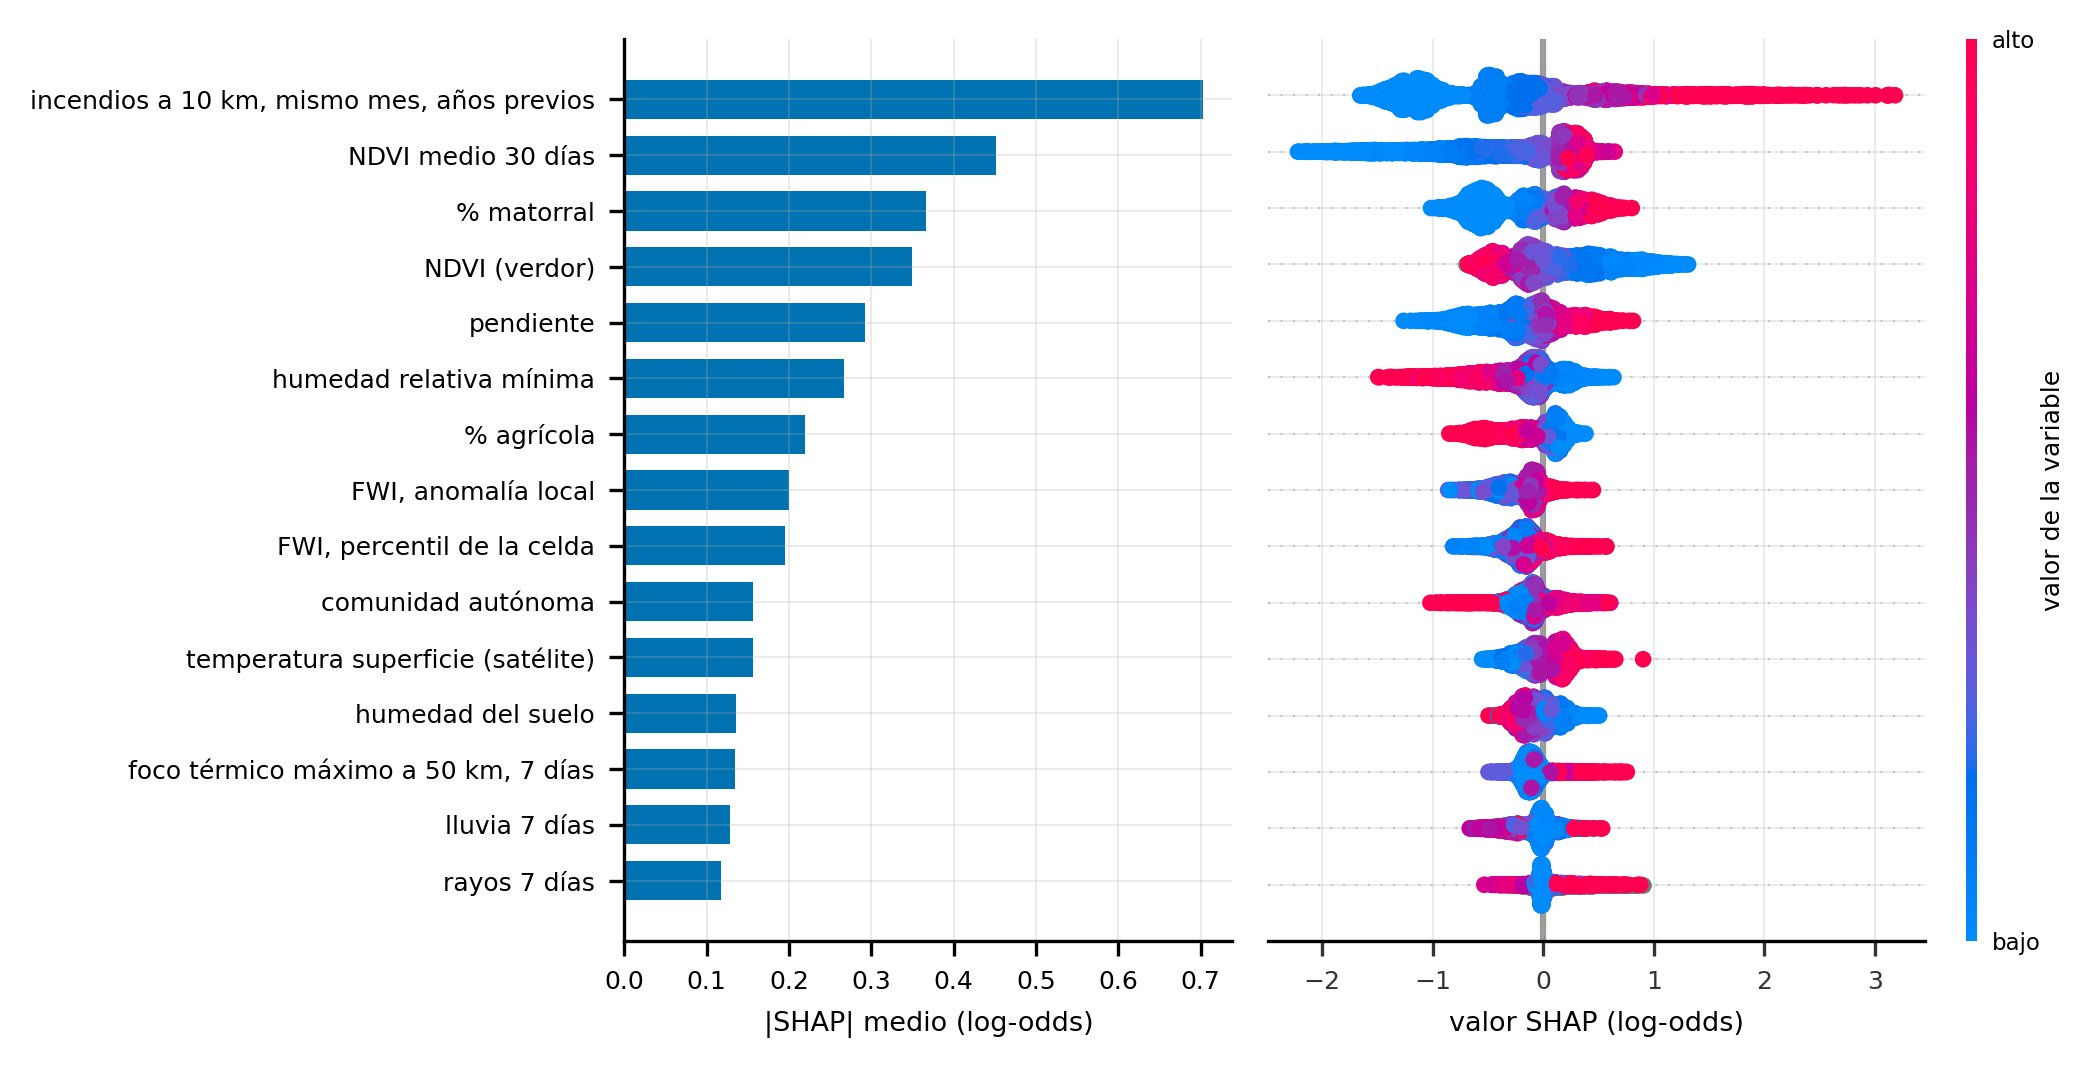
\includegraphics[width=.62\textwidth]{pagina_3_imagen_1_Im1.jpg}
  \caption{Variables en las que se apoya el r10: las 15 de mayor peso según
  los valores SHAP (\emph{SHapley Additive exPlanations}) sobre 6,000
  celdas-día de los veranos de 2023 y 2024, que el modelo no vio al entrenar.
  A la izquierda, la importancia media. A la derecha, el efecto de cada fila
  (a la derecha del cero eleva el riesgo), con el valor de la variable en color
  (rojo, alto). Historial de fuego, combustible y sequedad, por ese orden.}
  \label{fig:shap}
\end{figure}

\FloatBarrier
\subsection{Resultados, límites y conclusiones}

Para comparar los dos modelos en igualdad de condiciones se reprodujeron día a
día las temporadas de 2025 (del 1 de junio al 1 de noviembre) y de 2026 (hasta
el 2 de septiembre). Ambos modelos recibieron la previsión disponible la
víspera y se evaluaron con los perímetros de EFFIS. La tabla~\ref{tab:replay} recoge
los resultados.

\begin{table}[htbp]
  \centering
  \caption{Acierto medio por día (AUC dentro del día) del modelo de producción
  y del r10 con la previsión de la víspera, evaluados con EFFIS. La diferencia
  es la media pareada día a día, con IC (intervalo de confianza) bootstrap al
  95~\%.}
  \label{tab:replay}
  \scriptsize
  \begin{tabular}{lrrrrcr}
    \toprule
    Temporada & Días con fuego & Hectáreas & Producción & r10 & Diferencia (IC~95~\%) & Días que gana el r10 \\
    \midrule
    2025 & 138 & 387,000 & 0.743 & 0.807 & $+0.064$ [$+0.027$, $+0.101$] & 60~\% \\
    2026 &  86 & 268,000 & 0.658 & 0.762 & $+0.104$ [$+0.065$, $+0.144$] & 67~\% \\
    \bottomrule
  \end{tabular}
\end{table}

De la tabla se extraen tres lecturas. La primera: el
intervalo no incluye el cero en ninguna temporada, y el r10 gana dos de cada
tres días, con más ventaja en 2026, la temporada en la que el modelo de
producción obtuvo peores resultados.

La segunda: usar la previsión meteorológica de la víspera no supone un coste.
Cada día se calculó también con el tiempo realmente observado, y la diferencia
de AUC es de $-0.003$, con un intervalo que incluye el cero. El modelo no
depende de acertar el tiempo al detalle, sino de conocer dónde está el
combustible y cuánto tiempo lleva seco.

La tercera: el mapa indica dónde vigilar, no dónde va a arder. Que una celda
concreta arda un día concreto ocurre una vez de cada diez mil. El producto es
una herramienta de vigilancia, no una alarma por celda.

Queda por resolver cómo presentar el resultado. Durante la temporada el mapa
se pintó por posición en el ranking del día, con el 2~\% superior en rojo. Esa
regla señala dónde mirar, pero no cuánto riesgo hay: el ranking siempre tiene un
primero, de modo que un día de febrero muestra tanto rojo como el 15 de agosto.
Por ello se publican dos mapas del mismo modelo y una cifra
(figura~\ref{fig:escala}).

El primer mapa mantiene el percentil del día e indica las celdas prioritarias. El
segundo fija los colores en la escala de la puntuación del modelo. Los cortes se
obtuvieron de los 250 días de 2025 y 2026 calculados con la cadena de servicio,
de forma que el nivel extremo reúne el 2~\% de las celdas-día más altas de ese
periodo. En ese nivel ardió una de cada 760 celdas-día, 13 veces la media de las
dos temporadas (anexo~C).

En la escala absoluta la cantidad de rojo cambia de un día a otro: el 13 de
agosto de 2025 cubrió el 4.8~\% de España y el 29 de octubre, el 0.3~\%. Como
la diferencia no siempre se aprecia a simple vista, el mapa se acompaña de una
cifra: el porcentaje de España en nivel extremo y su posición entre los días de
referencia. La cifra resume cuánto riesgo marca el mapa, pero anticipa con
cautela los días con incendio grande: en 2025 y 2026 obtuvo un AUC de 0.69 y
0.66, frente a 0.74 y 0.44 del calendario.

La puntuación no es una probabilidad, sino un valor para ordenar y
comparar con la historia.

\begin{figure}[htbp]
  \centering
  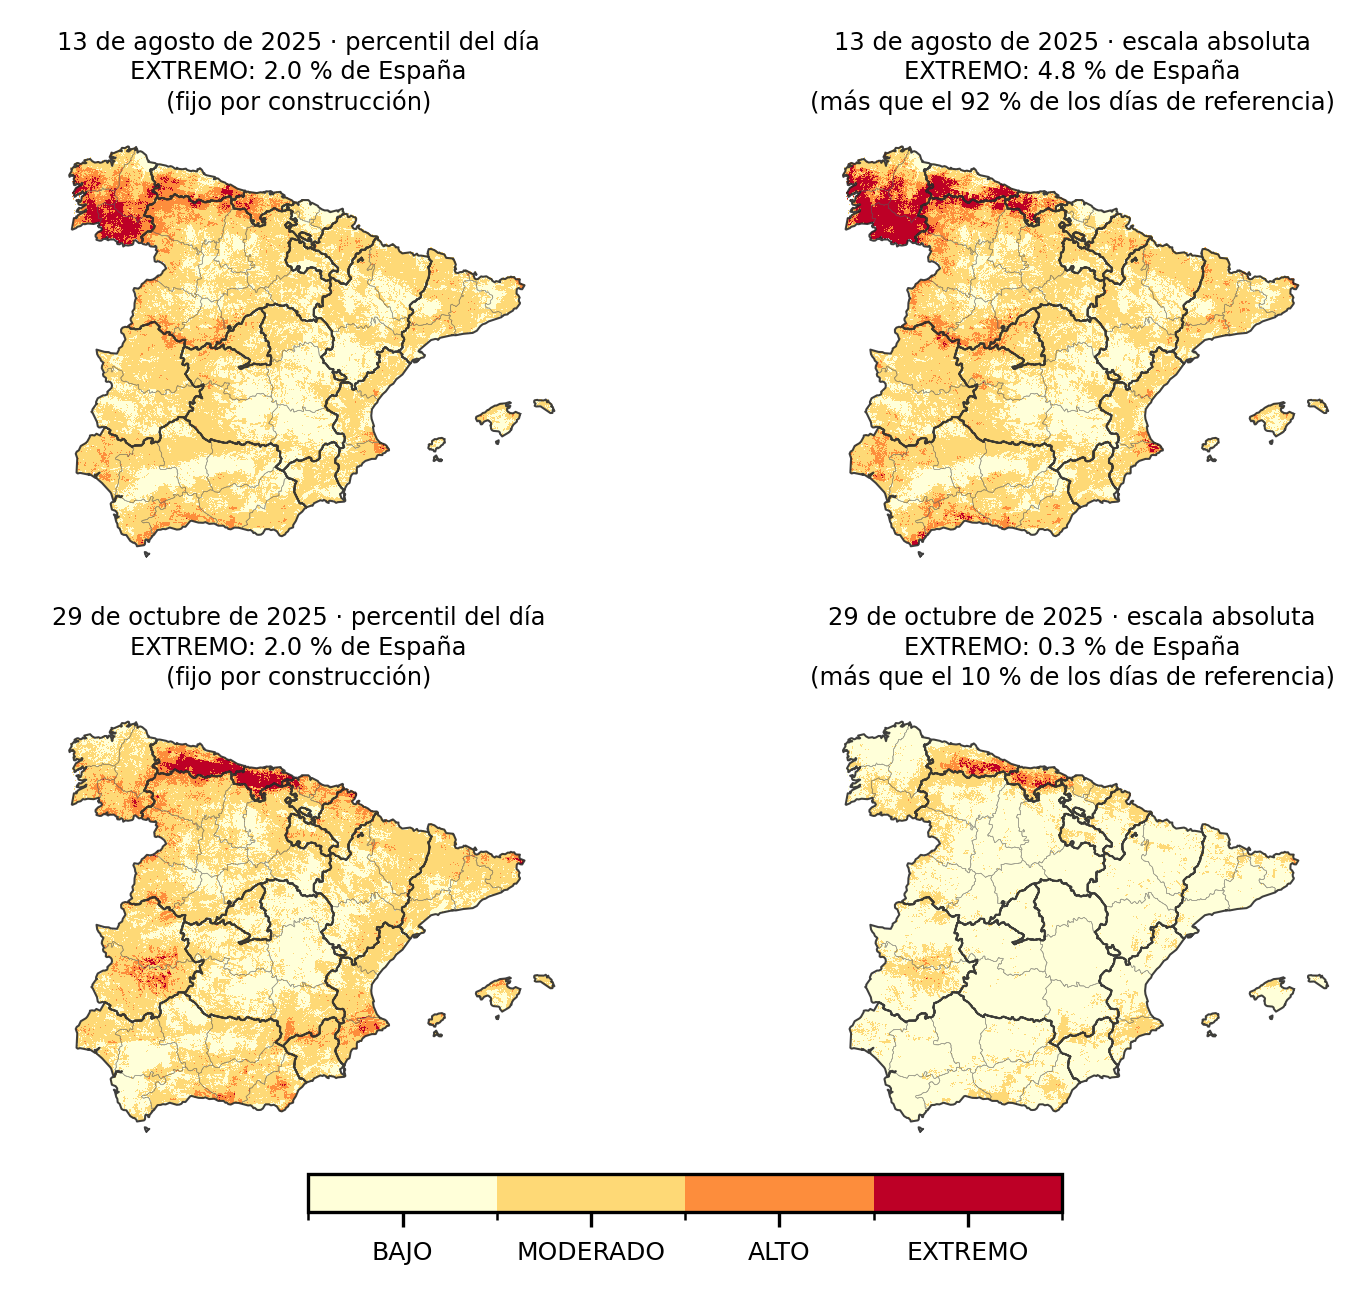
\includegraphics[width=.62\textwidth]{fig3_dos_mapas.png}
  \caption{El mismo modelo (r10) en un día de pleno verano (13 de agosto de 2025,
  arriba) y en uno fuera de temporada (29 de octubre de 2025, abajo). Izquierda:
  niveles por percentil del día, que asignan el 2~\% de extremo todos los días.
  Derecha: cortes fijos en la escala de la puntuación y la cifra del día, es
  decir, el porcentaje de España en extremo y su posición entre los días de
  referencia. Los días de referencia son los 250 días de las temporadas de 2025
  (del 25 de mayo al 1 de noviembre) y de 2026 (del 25 de mayo al 2 de
  septiembre), calculados igual que el mapa diario; de ellos salen también los
  cortes.}
  \label{fig:escala}
\end{figure}
\FloatBarrier

La propuesta tiene tres límites. La evaluación de las dos temporadas es a
posteriori: los mapas usan la previsión de cada víspera, pero se generaron
después y no se publicaron día a día. La escala absoluta se calibró con 250 días de temporada, sin datos de diciembre a
abril, y su referencia debe ampliarse con cada día publicado. Y la cobertura se limita a la Península y
Baleares, sin Canarias, con datos de 2026 hasta el 2 de septiembre.

Como conclusión, un modelo se optimiza para la pregunta que define su conjunto
de entrenamiento. Esa pregunta la determinan la elección de positivos y
negativos, no la intención de quien lo entrena. Un acierto alto sobre un
conjunto de prueba construido con el mismo diseño que el de entrenamiento no
garantiza nada sobre el uso previsto. Por ello, en la segunda iteración se
evaluó cada día con la misma verdad con la que se entrena.

La utilidad del resultado se aprecia en la temporada completa de 2025 con el
r10. Con un radio operativo de 6~km, se cubrió el 44~\% de los incendios
vigilando cerca del 10~\% del territorio. Es un resultado notable en un
fenómeno en el que, en verano, arden entre 2 y 7 celdas de cada 100,000 al día. Esa
cobertura permite concentrar la vigilancia en las zonas señaladas, por
ejemplo con visión artificial desde cámaras o drones. Permite también avisar
a la población y desplegar recursos de forma preventiva, y reducir así el
impacto económico, social y humano de los incendios forestales.

El código, con cada cifra enlazada al script que la produjo, está disponible
en el repositorio (anexo~D).


% ============================================================================
%                                   ANEXOS
% ============================================================================
\clearpage
\section*{Anexos}
\renewcommand{\thesubsection}{\Alph{subsection}}
\renewcommand{\theHsubsection}{anexo.\Alph{subsection}}
\setcounter{subsection}{0}
\newcommand{\repo}[2]{\href{https://github.com/JuanUtrilla/tfm-riesgo-incendios/#1}{\texttt{#2}}}

Estos anexos recogen solo las tablas y figuras imprescindibles. El detalle de cada parte,
con los scripts que produjeron cada cifra, está en el repositorio del trabajo
(anexo~D).

\subsection{Datos}

Además de las cuatro fuentes del apartado de datos, se usaron la observación de
687 estaciones de AEMET (meteorología del primer modelo en producción), los focos
térmicos de FIRMS (variables de fuego reciente) y los partes del MITECO (segunda
referencia durante el desarrollo).

La figura~\ref{fig:an-prev} resume las dos propiedades de los datos que más
condicionaron el diseño. La primera es la escasez: en verano arden entre 0.5 y
38 celdas de cada 100,000 al día, según el año, frente al 25~\% de positivos
del conjunto de la primera iteración. La segunda es la persistencia de la
etiqueta de EFFIS: una celda que arde un día sigue marcada al siguiente con
probabilidad 0.51, así que las evaluaciones cuentan solo el primer día de cada
celda quemada.

\begin{figure}[H]
  \centering
  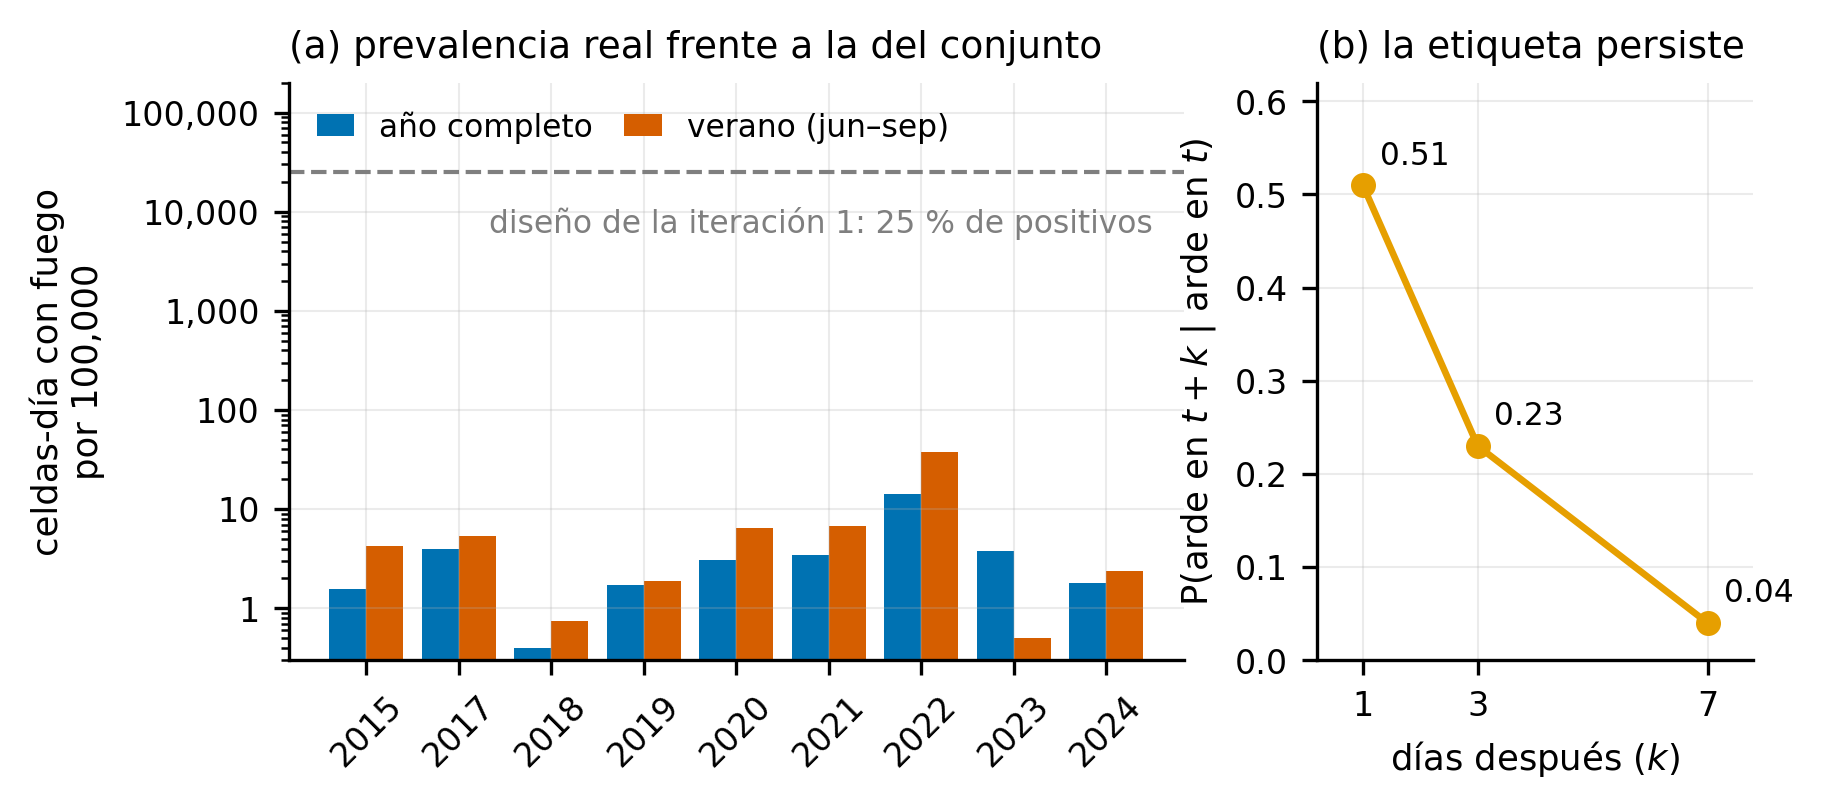
\includegraphics[width=.66\textwidth]{anexo_a_prevalencia.png}
  \caption{(a)~Celdas-día con fuego por cada 100,000, año completo y verano, en
  escala logarítmica, frente a la proporción de positivos del primer diseño.
  (b)~Probabilidad de que una celda siga marcada como quemada $k$ días después.}
  \label{fig:an-prev}
\end{figure}

Las 46 variables y su orden están en
\repo{blob/main/01_datos/comun/features.py}{01\_datos/comun/features.py}; la
descarga y el tratamiento de cada fuente, en
\repo{blob/main/01_datos/README.md}{01\_datos/README.md}.

\subsection{Benchmark y alternativas descartadas}

La figura~\ref{fig:an-benchmark} compara los
seis modelos de la reproducción de 2025 y 2026, con la previsión de la víspera.
Los dos modelos únicos encabezan las dos temporadas; la pareja supera a
producción, pero queda por debajo; el modelo de «dónde» por separado no se
distingue de producción y el de «cuándo» queda por debajo. La
tabla~\ref{tab:an-descartes} resume las alternativas al r10 que no se
adoptaron.

\begin{figure}[H]
  \centering
  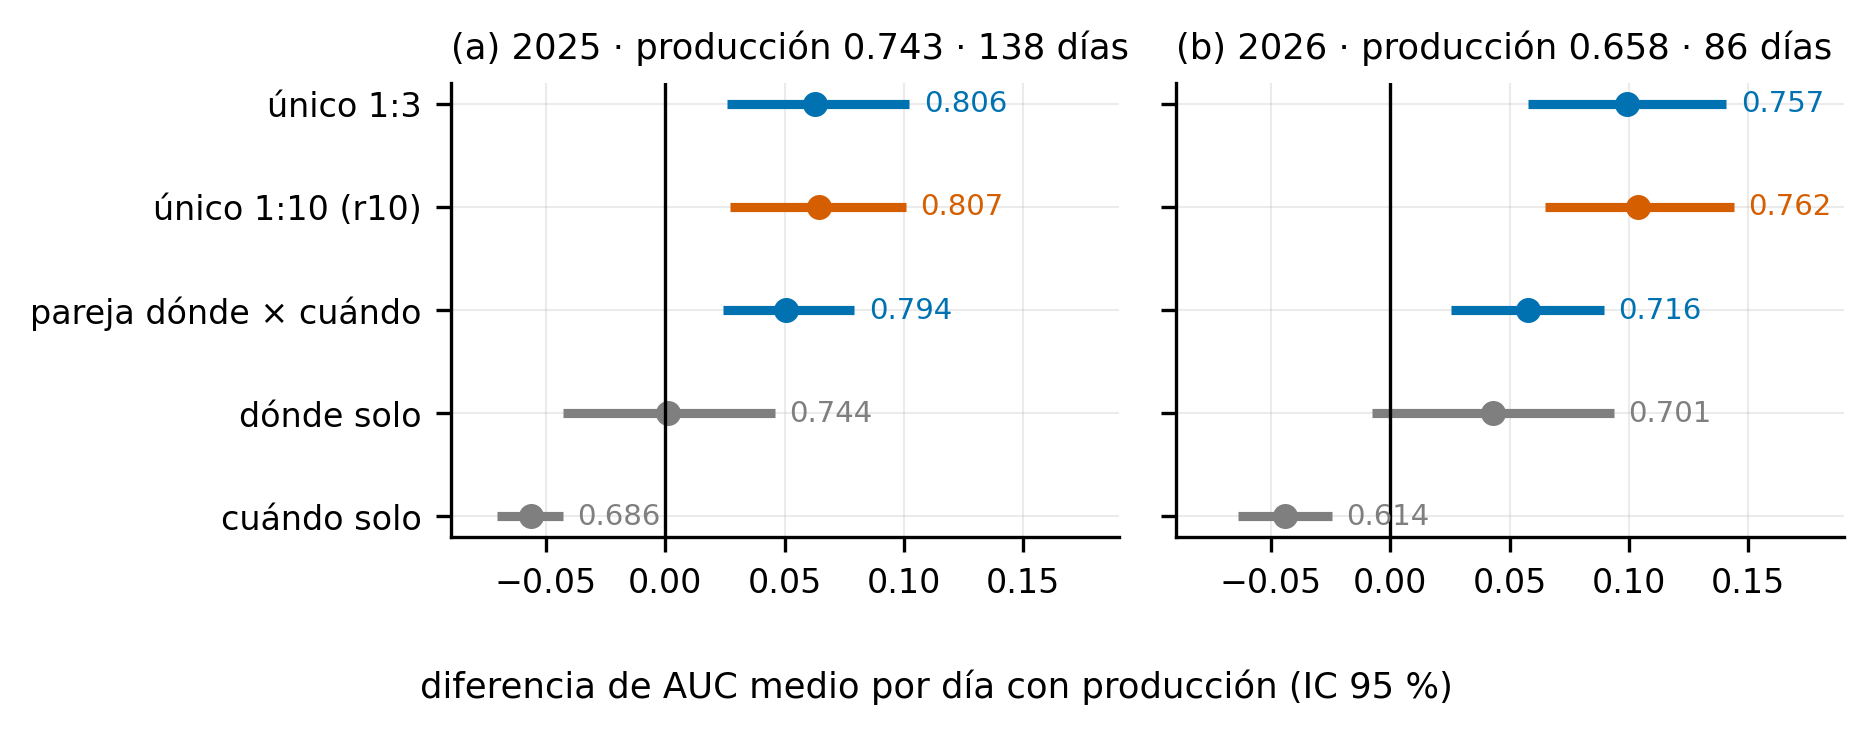
\includegraphics[width=.72\textwidth]{anexo_b_replay.png}
  \caption{Diferencia de AUC medio por día de cada modelo con producción, con su
  IC al 95~\%. A la derecha de cada barra, el AUC medio del modelo. En rojo, el
  r10; en gris, los intervalos que incluyen el cero.}
  \label{fig:an-benchmark}
\end{figure}

En superficie, el r10 situó en el 10~\% de celdas de mayor riesgo de cada día el
63.0~\% de las hectáreas quemadas en 2025 y el 37.0~\% en 2026, frente al 59.6 y
24.7~\% de producción. La pareja captó más superficie en 2025 (72.4~\%) y menos en
2026 (23.7~\%).

\begin{table}[H]
  \centering
  \caption{Alternativas descartadas. Diferencia de AUC medio por día con la
  configuración de referencia de cada prueba.}
  \label{tab:an-descartes}
  \footnotesize
  \begin{tabular}{@{}>{\raggedright}p{5.4cm}>{\raggedright\arraybackslash}p{10.8cm}@{}}
    \toprule
    Alternativa & Resultado \\
    \midrule
    De 1:3 a 1:100 negativos por positivo & AUC de 2026 entre 0.745 y 0.759; el percentil ponderado por hectáreas fue máximo con 1:10 (81.9) \\
    Entrenar solo con verano & Entre $-0.011$ y $-0.041$ en cuatro conjuntos de prueba \\
    Apagar las celdas quemadas en los 7 a 60 días previos & Entre $-0.017$ y $-0.027$ en la temporada de 2026 \\
    Reentrenar el r10 con 2015--2024 & $+0.0033$ [$-0.0042$, $+0.0104$]: sin mejora \\
    \bottomrule
  \end{tabular}
\end{table}

La reproducción completa, con la captura de hectáreas y el lift, está en
\repo{blob/main/06_comparacion/README.md}{06\_comparacion/README.md} y
\repo{blob/main/docs/REPLAY_CAPTURA.md}{docs/REPLAY\_CAPTURA.md}; las
alternativas, en \repo{blob/main/05_iteracion2/README.md}{05\_iteracion2/README.md}.

\subsection{Escala absoluta y cifra del día}

Los cortes de la escala absoluta se obtuvieron de los 250 días de referencia,
calculados igual que el mapa diario. Los cortes calculados con los diez años del
cubo marcaban en esos mapas entre dos y diez veces más celdas en extremo que el
cubo en el mismo mes. La tabla~\ref{tab:an-niveles} da el significado de cada
nivel.

\begin{table}[H]
  \centering
  \caption{Niveles del r10 en los 250 días de referencia. Factor: frecuencia de
  quema del nivel dividida entre la media.}
  \label{tab:an-niveles}
  \footnotesize
  \begin{tabular}{@{}lrrrrr@{}}
    \toprule
    Nivel & Corte & Celdas-día (\%) & Una quemada de cada & Factor & Hectáreas (\%) \\
    \midrule
    BAJO     & 0      & 30.0 & 132,600 & 0.08  & 1.5  \\
    MODERADO & 0.0060 & 60.0 & 14,200  & 0.71  & 40.0 \\
    ALTO     & 0.1125 & 8.0  & 2,760   & 3.63  & 29.5 \\
    EXTREMO  & 0.4058 & 2.0  & 760     & 13.17 & 29.0 \\
    \bottomrule
  \end{tabular}
\end{table}

La cifra del día sitúa el porcentaje de España en extremo entre esos 250 días,
cuya mediana es el 1.5~\% y cuyo percentil 90 es el 4.6~\%. Para separar los días
con incendio grande obtuvo un AUC de 0.69 en 2025 y de 0.66 en 2026, frente a
0.74 y 0.44 del calendario. Los cortes deben recalcularse al acumular días
publicados, en especial de diciembre a abril. El detalle, junto con el semáforo
nacional que se evaluó y se descartó, está en
\repo{blob/main/07_produccion/escala_y_cifra/README.md}{07\_produccion/escala\_y\_cifra/README.md}.

\subsection{Limitaciones y repositorio}

\begin{table}[H]
  \centering
  \caption{Limitaciones principales.}
  \label{tab:an-limitaciones}
  \footnotesize
  \begin{tabular}{@{}>{\raggedright}p{3.6cm}>{\raggedright\arraybackslash}p{12.6cm}@{}}
    \toprule
    Limitación & Efecto \\
    \midrule
    Evaluación a posteriori & Los mapas de 2025 y 2026 usan la previsión de cada víspera, pero se generaron después; el protocolo se escribió antes de ejecutarlos \\
    Escala absoluta & Calibrada con 250 días de temporada, sin diciembre a abril; con cortes de 2025, en 2026 el extremo pasó de una celda quemada de cada 550 a una de cada 2,560 \\
    Variables de vecindad & En el mapa diario son entre un 36 y un 54~\% mayores que al entrenar; cambian la escala, no el orden de las celdas \\
    Incertidumbre & El sorteo de negativos mueve el AUC 0.004; los IC suponen días independientes y son una cota inferior \\
    Probabilidad por celda & Depende de la intensidad de la temporada (en julio, del 0.00~\% en 2023 al 12.76~\% en 2022); se publican niveles \\
    Cobertura & Península y Baleares, sin Canarias, Ceuta ni Melilla; datos de 2026 hasta el 2 de septiembre \\
    \bottomrule
  \end{tabular}
\end{table}

El repositorio
(\href{https://github.com/JuanUtrilla/tfm-riesgo-incendios}{\texttt{github.com/JuanUtrilla/tfm-riesgo-incendios}})
sigue el orden de esta memoria. Cada carpeta tiene un \texttt{README.md} con lo
que hace cada script y para qué se usó (tabla~\ref{tab:an-repo}).

\begin{table}[H]
  \centering
  \caption{Dónde ampliar cada parte de la memoria.}
  \label{tab:an-repo}
  \footnotesize
  \begin{tabular}{@{}>{\raggedright}p{5.4cm}>{\raggedright\arraybackslash}p{10.8cm}@{}}
    \toprule
    Parte & Enlace \\
    \midrule
    Datos y análisis exploratorio & \repo{tree/main/01_datos}{01\_datos} · \repo{tree/main/02_eda}{02\_eda} \\
    Primer modelo y diagnóstico & \repo{tree/main/03_iteracion1}{03\_iteracion1} · \repo{tree/main/04_bisagra}{04\_bisagra} \\
    Segundo modelo y calibración & \repo{tree/main/05_iteracion2}{05\_iteracion2} · \repo{tree/main/05_iteracion2/56_calibracion}{05\_iteracion2/56\_calibracion} \\
    Reproducción de 2025 y 2026 & \repo{tree/main/06_comparacion}{06\_comparacion} · \repo{blob/main/docs/REPLAY_VEREDICTO.md}{docs/REPLAY\_VEREDICTO.md} \\
    Mapa diario, escala y cifra & \repo{tree/main/07_produccion}{07\_produccion} · \repo{tree/main/07_produccion/escala_y_cifra}{07\_produccion/escala\_y\_cifra} \\
    Cifra a cifra: script y fichero de origen & \repo{blob/main/docs/TRAZABILIDAD.md}{docs/TRAZABILIDAD.md} \\
    Procedencia de cada fichero & \repo{blob/main/docs/PROCEDENCIA.md}{docs/PROCEDENCIA.md} \\
    \bottomrule
  \end{tabular}
\end{table}

\end{document}
